Due to the numerous processes associated with the deep carbon cycle, precise quantitaive measurements over the lifetime of Earth are lacking. Therefore, simpliyfing the model to the basic set of reservoirs and/or fluxes is vital otherwise the results maybe meaningless. 

In order to test our hypothesis, we construct a reservoir model taking into consideration some of the constraints opting for simplicity due to the numerous uncertainities revolving around the carbon cycle. First, we examine the mantle reservoir. We do not take into consideration the core in our reservoir model as there is little to no evidence of transport of carbon between the core and the mantle. Next, we consider the whole mantle as a homogeneous reservoir. Since we are modeling the solid Earth carbon cycle, we do not take into account any of the surficial reservoirs and associated fluxes excluding the atmosphere. The abundances of carbon are taken from \citet{KLH-TDL-WM:2017} and are shown in Table.~\ref{Table:Masses of carbon in Earth's reservoirs}.

\begin{figure}
  \centering
  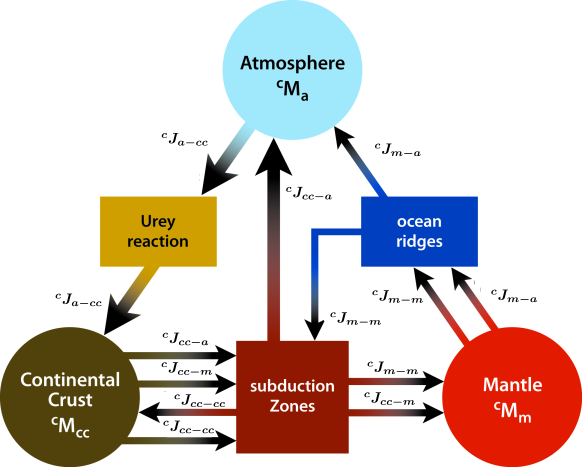
\includegraphics[scale=0.5]{Figures/RelabelJaniceFlowDiagram.png}
  \caption{A flow diagram showing the different reservoirs and pathways in our constructed box model.}
  \label{ReservoirFlowDiagram}
\end{figure}


We first consider the mantle reservoir. We assume that carbon can be added to the mantle from the atmosphere early in Earth's history. This is the hypothesis set forth by Sleep and Zahnle (2001). Since little is known about the time dependence of this process we assume that the rate of mass addition decays exponentially with the age of the Earth. We also assume there is no significant transfer of carbon between the mantle and continental crustal reservoirs. This is consistent with association of carbon in the continental crustal reservoir and carbon in the atmosphere.

With these assumptions the mass of carbon in the mantle reservoir $^cM_{m}(t)$ is given as a function of time by

\begin{equation}
  ^cM_{m}(t) = ^cM_{m0} + (^cM_{mp} - ^cM_{m0}) (1 - e^{-\frac{t}{\tau_{am}}})
\end{equation}

where time is measured forward from the time of core formation ($t=0$) to the present ($t=4.4$ Gyr). The initial mass of carbon in the mantle is $^cM_{m0}$, the present mass of carbon in the mantle is $^cM_{mp}$, and the time constant for the loss of carbon from the atmosphere to the mantle is $\tau_{am}$. There is considerable uncertainty in the value of $\tau_{am}$ but on the basis of our previous discussion we take $\tau_{am} = 2 \times 10^8$ yrs.

We also require that the total mass of carbon in the three large reservoirs be constant over time. This balance between $t=0$ and $t_p$, requires that

\begin{equation}
  ^cM_{m0} = ^cM_{mp} + ^cM_{ccp} - ^cM_{a0}
\end{equation}

where $^cM_{a0}$ is the mass of carbon in the atmosphere at $t=0$ and $^cM_{ccp}$ is the mass of carbon in the continental crust at $t=t_p$. The continental crust did not exist at $t=0$ so that $^cM_{cc0}=0$. As we have discussed the present mass of carbon in the atmosphere is negligible compared with the carbon masses in the mantle and the continental crust so that it is appropriate to take $^cM_{ap}=0$ in our mass balance. Eliminating $^cM_{m0}$ we obtain an expression for the mass of carbon in the mantle as a function of time

\begin{equation}
  ^cM_{m}(t) = ^cM_{mp} + ^cM_{ccp} - ^cM_{a0} + (^cM_{a0} - ^cM_{ccp}) (1 - e^{-\frac{t}{\tau_{am}}})
\end{equation}

To obtain the dependence of $^cM_{m}$ on time we must specify $^cM_{mp}$, $^cM_{ccp}$, $^cM_{a0}$, and $\tau_{am}$.


We next consider the continental crust reservoir. Our approach is based on the hypothesis that carbon in the continental crust was primarily extracted from the atmosphere through the application of the Urey equation shortly after the first formation of continental crust. We specify that the continental crust began to form at $t=t_{cc0}$. Prior to this time there was no carbon in the continental crust so that

\begin{equation}
  ^cM_{cc} = 0 \quad \text{for} \quad 0 < t < t_{cc0}
\end{equation}

For our analysis of the evolution of major carbon reservoirs we assume that at $t=t_{cc0}$ the mass of carbon in the atmosphere was equal to the present mass of carbon in the continental crust $^cM_{ccp}$. We model the loss of carbon from the atmosphere with the growth equation

\begin{equation}
    \frac{d ^cM_{cc}(t)}{d t} = \frac{1}{\tau_{acc}} [^cM_{ccp} - ^cM_{cc}(t)]
\end{equation}

which is valid for the period $t_{cc0} < t < t_p$ and has the initial condition $^cM_{cc} = 0$ at $t = t_{cccp}$. The applicable solution of the growth equation is

\begin{equation}
    ^cM_{cc}(t) = ^cM_{ccp} (1 - e^{-\frac{(t-t_{cc0})}{\tau_{acc}}} )
\end{equation}

The mass of carbon in the continental crust grows exponentially with a time constant $\tau_{acc}$.

Finally we consider the atmosphere reservoir. As previously stated the sum of the carbon masses in the three large reservoirs is constant. We first consider the time period $0 < t < t_{cc0}$. During this period we have $^cM_{cc}=0$ so that we can write

\begin{equation}
    ^cM_{a}(t) = ^cM_{a0} + ^cM_{m0} - ^cM_{m}(t)
\end{equation}

since we require that the total mass of carbon in the three large reservoirs be constant over time between $t=0$ and $t_p$,

\begin{equation}
  ^cM_{a0} + ^cM_{m0} = ^cM_{mp} + ^cM_{ccp}
\end{equation}

substitution gives 

\begin{equation}
    ^cM_{a}(t) = ^cM_{mp} + ^cM_{ccp} - ^cM_{m}(t)
\end{equation}

and substitution of $^cM_{m}$(t) gives

\begin{equation}
    ^cM_{a}(t) = ^cM_{a0} - (^cM_{a0} - ^cM_{ccp})(1 - e^{\frac{-t}{\tau_{ca}}})
\end{equation}

for the period $0 < t < t_{cc0}$.

We next consider the time period $t_{cc0} < t < t_{p}$. During this period a mass balance gives

\begin{equation}
    ^cM_{a}(t) = ^cM_{mp} - ^cM_{m} (t) + ^cM_{ccp} - ^cM_{cc} (t)
\end{equation}

since for the large reservoir carbon mass balance we can take $^cM_{ap} = 0$. Substitution of $^cM_{m}(t)$ and substitution of $^cM_{cc}(t)$ gives

\begin{equation}
    ^cM_{a}(t) = (^cM_{a0} - ^cM_{ccp})e^{-\frac{t}{\tau_{am}}} + ^cM_{ccp} e^{-\frac{(t-t_{cc0})}{\tau_{acc}}}
\end{equation}

for the period $t_{cc0} < t < t_p$.


